\chapter{The Factory}
The Factory is a separate project that represents a business model with certain needs for the business
to succeed and make profits.\\\\
The business model involves business processes that are the core of this business. These processes
include
\begin{itemize}
    \item Manufacturing the products
    \item Warehousing
    \item Provide an online market to show the products and sell them
    \item Delivering the products to the customers
\end{itemize}

The Factory is made as a prototype of a business that wants to include technologies in their business
like
\begin{itemize}
    \item IOT
    \item Factory 4.0
    \item Provide an online market to show the products and sell them
    \item Delivering the products to the customers
\end{itemize}

The main purpose of The Factory project is to show a migration of an existing business with an
already working business model with The ERP and The BPM and how the business benefits by
migrating the business with our solutions.\\\\
We will first discuss The Factory as a separate project, its components, and how it works. Then we
will have a look at how migration can be done.\\\\
A flow diagram that shows how The Factory works in a separate matter Fig \ref{fig:factory_flow}

\begin{figure}[h]
    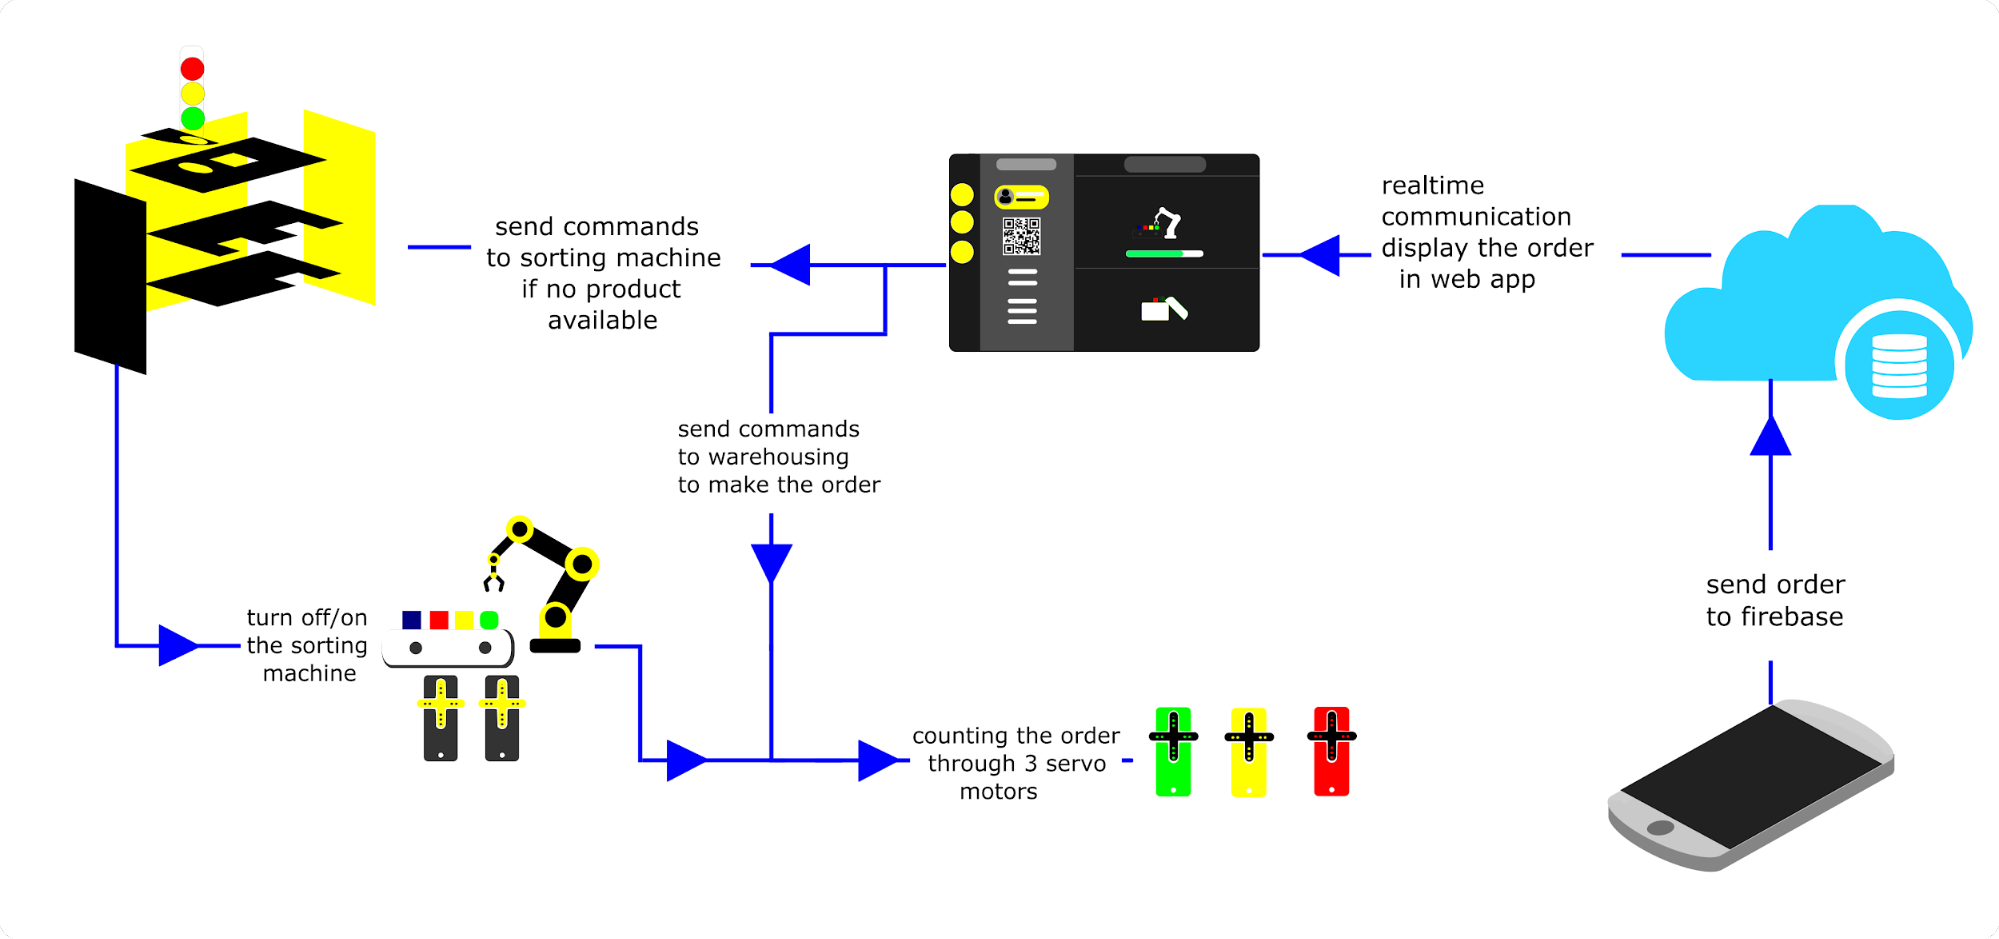
\includegraphics[width=100mm]{factory_flow}
    \centering
    \caption{The Factory Flow}
    \label{fig:factory_flow}
\end{figure}


\chapter{Hardware}

\section{Factory box Design}
We made all the factory box from black and yellow acrylic sheet with thickness 3 mm with a press fit
design to make assembling easier.\\
First, there are many programs used to make 3d designs like SolidWorks or Inventor but we used
CorelDRAW 2d program. It is a vector graphics editor that exports DXF files that the CNC machine
uses to execute the design.\\
It consists of three main parts. Fig \ref{fig:hard1}
\begin{itemize}
    \item Sorting part
    \item Warehousing part
    \item Collecting part
\end{itemize}

\begin{figure}[h]
    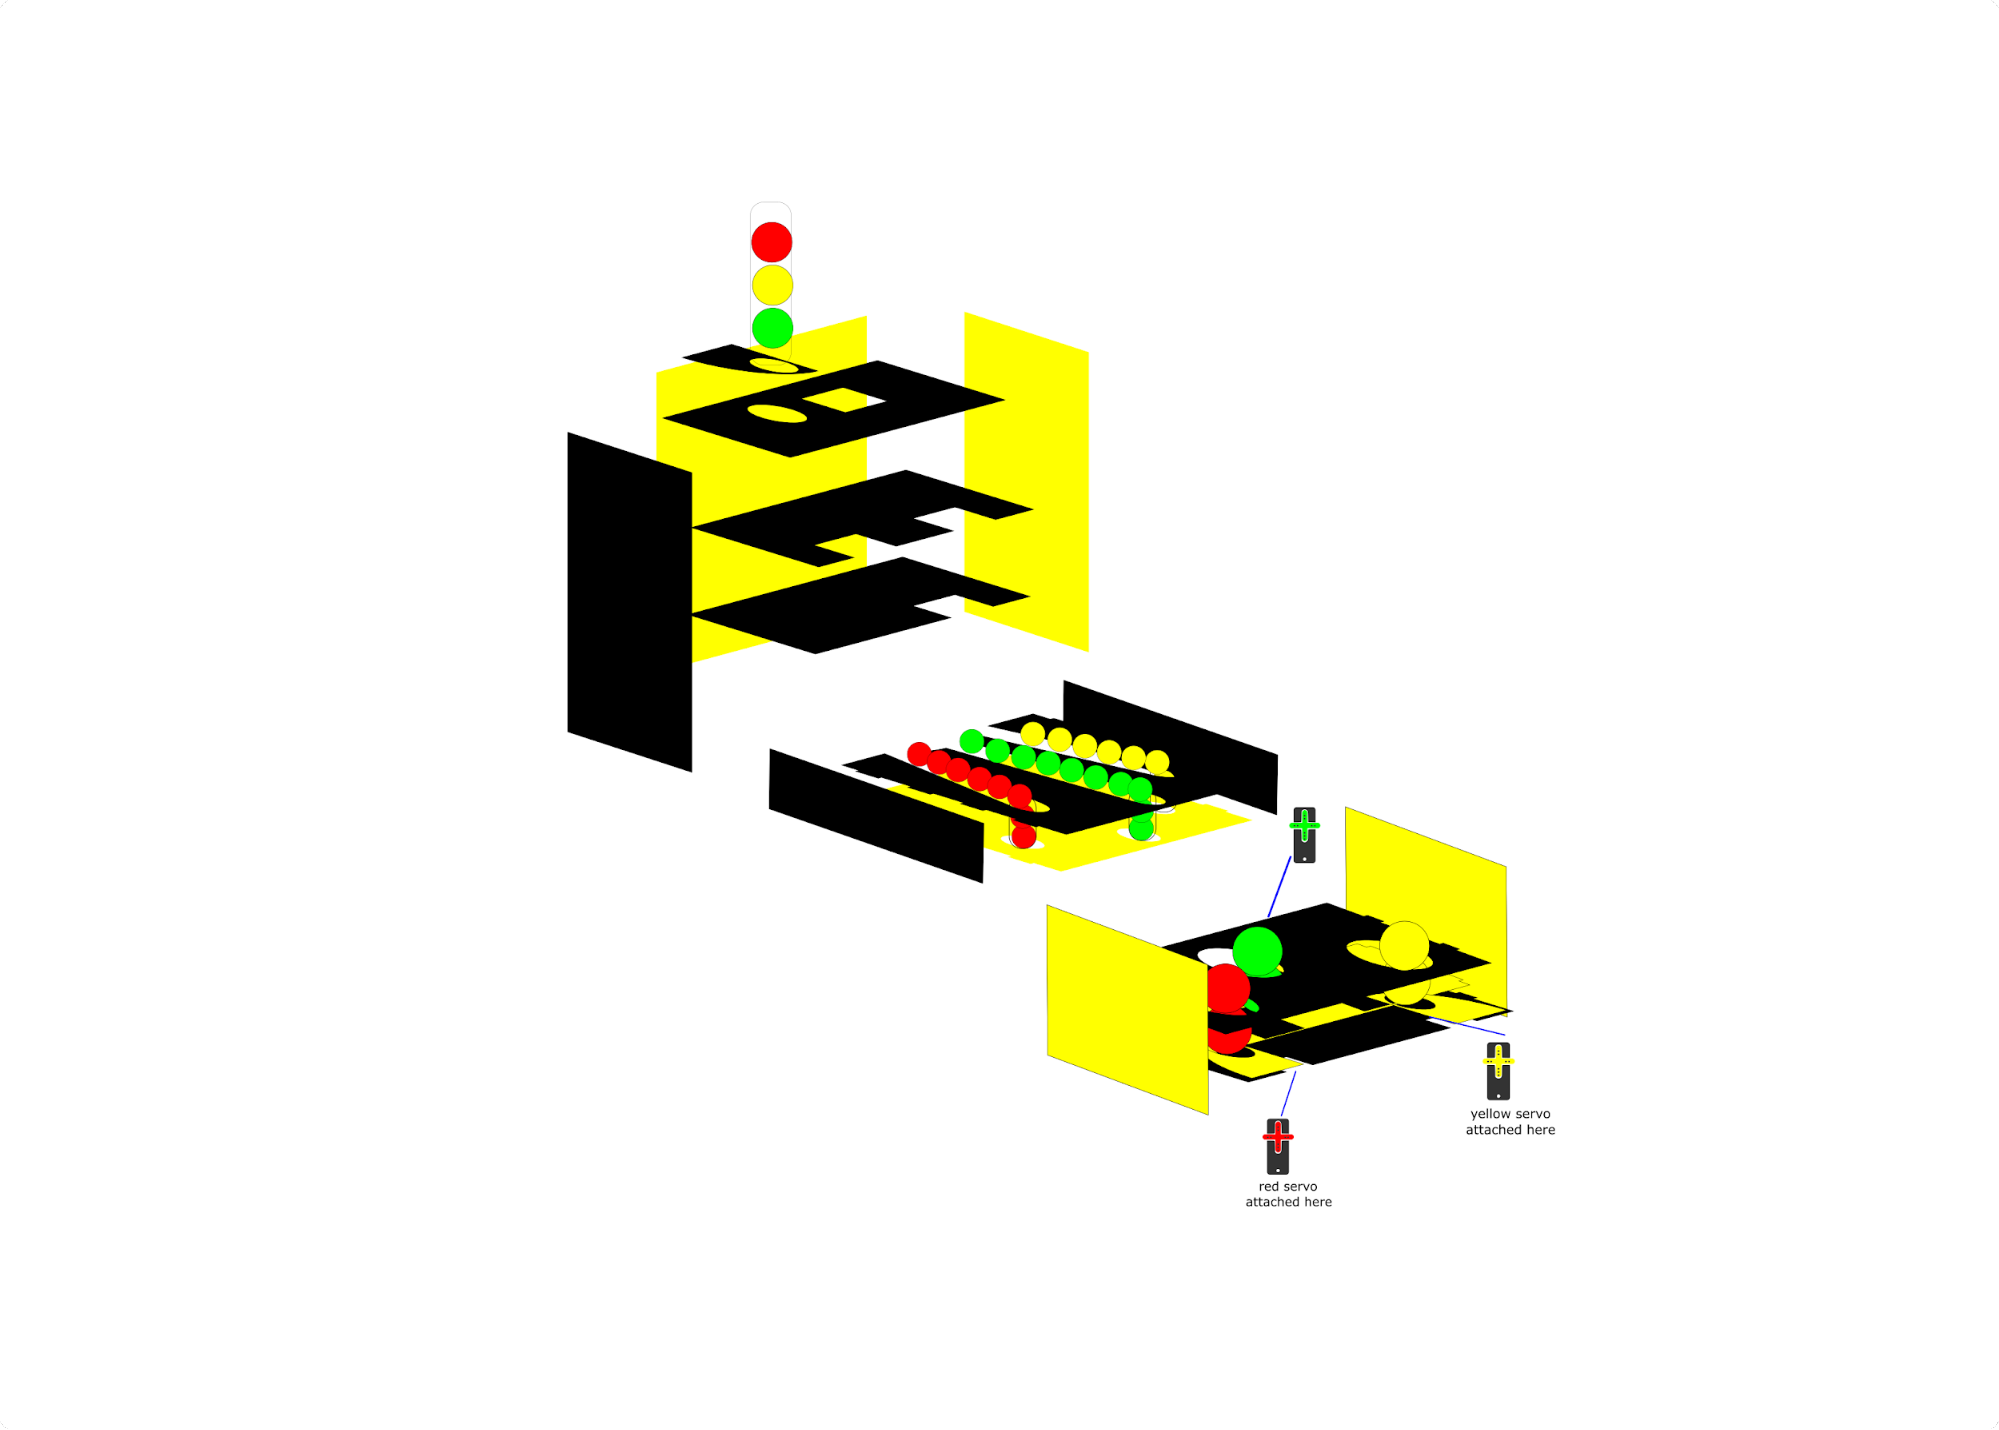
\includegraphics[width=105mm]{hard1}
    \centering
    \caption{Factory Box}
    \label{fig:hard1}
\end{figure}

\subsection{The sorting part}
This part is considered the first stage of our factory. The aim of this part is to make sorting to our
spherical products (colored ball) based on their colors then put them in a fixed place to bring them
quickly.\\
The base of this frame is a (10 cm * 15 cm) and the height is 30 cm.\\
It has 2 servo motors (upper and lower) and one color sensor. The upper servo takes the ball from the
cylindrical tube to put it below the sensor, so the sensor detects its color and the lower servo moves
the ball to the second stage in a specific route. Fig \ref{fig:hard2}

\begin{figure}[h]
    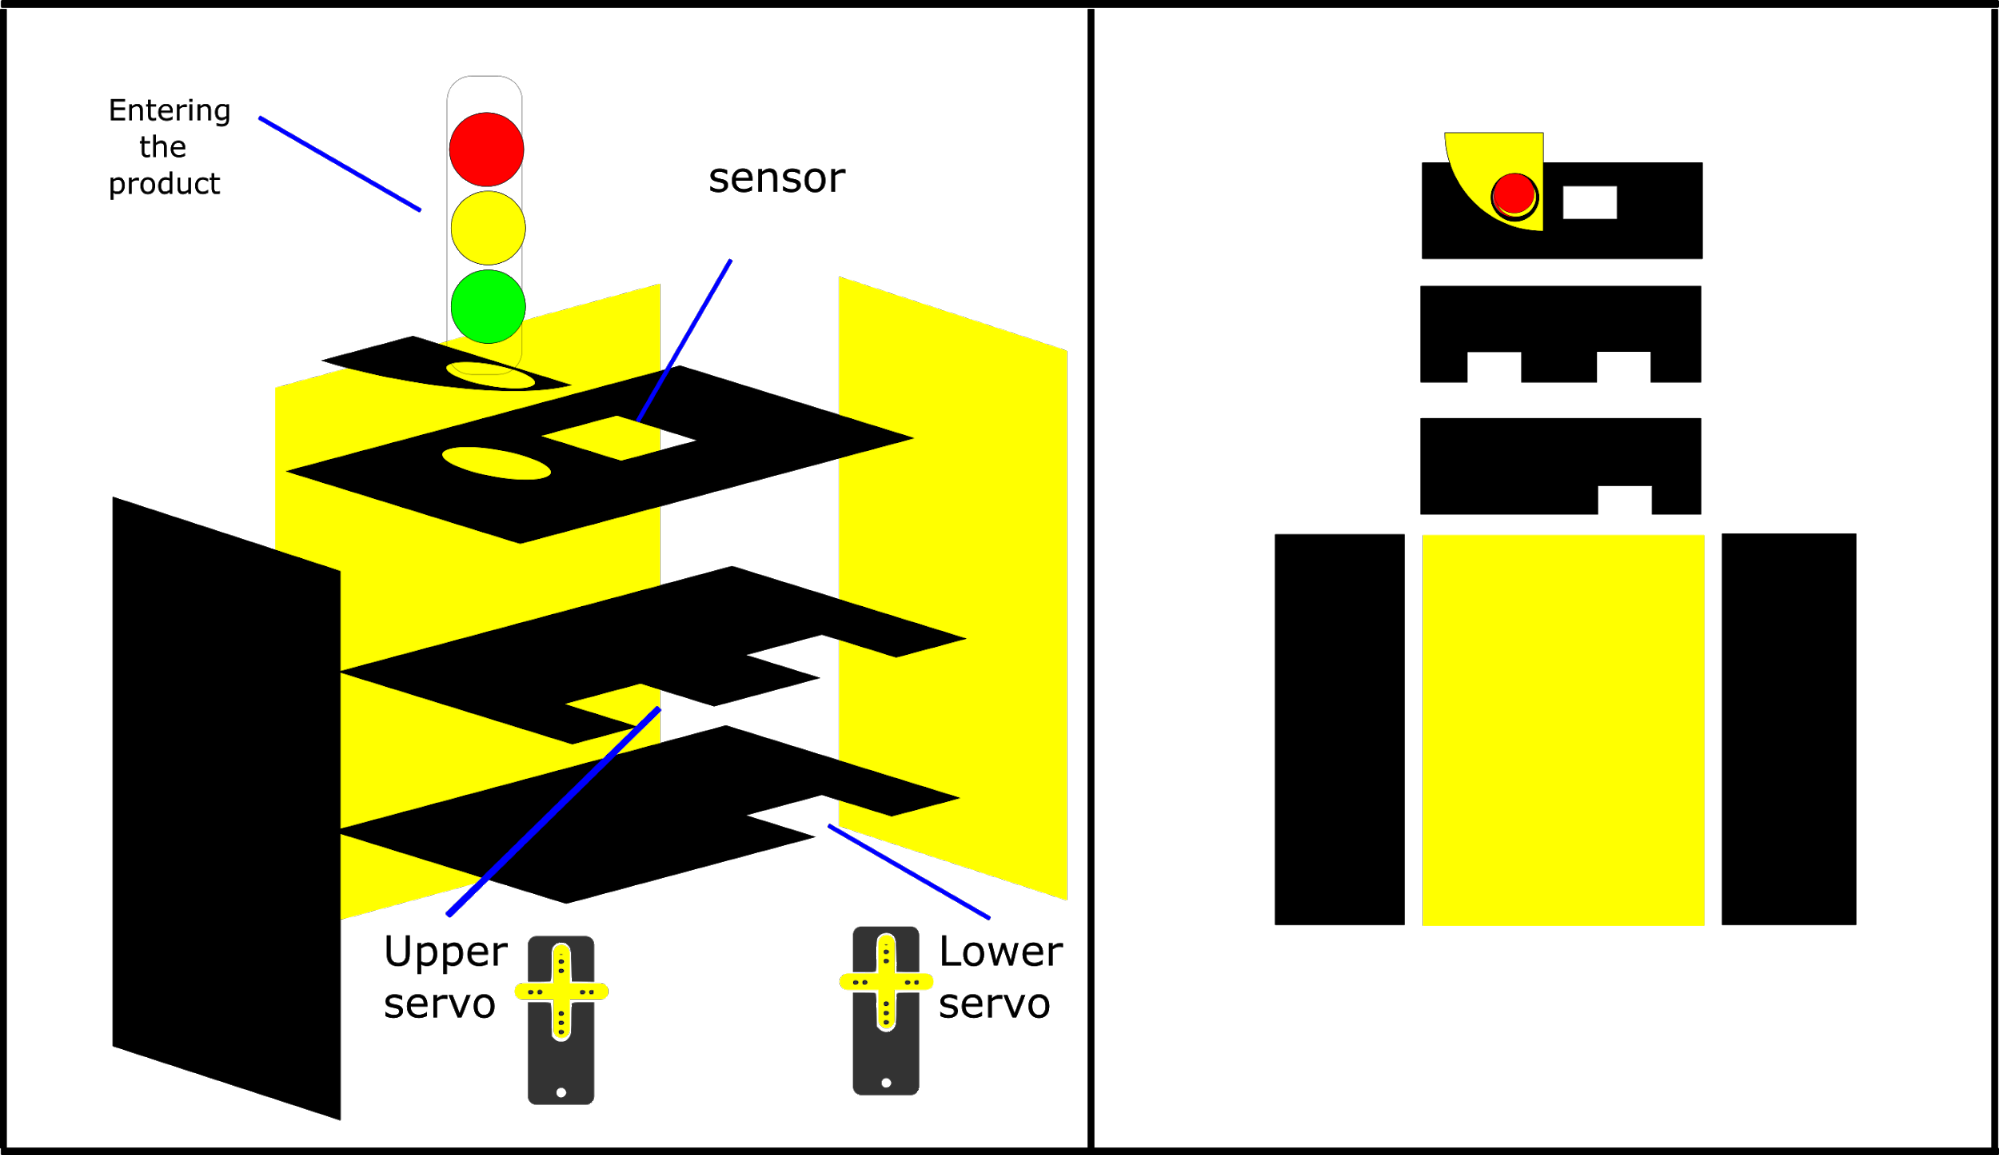
\includegraphics[width=100mm, height= 50mm]{hard2}
    \centering
    \caption{Sorting Part}
    \label{fig:hard2}
\end{figure}


\subsection{Warehousing part}
This part is considered the second stage. The aim of this part is to store the balls in a specific route
based on their colors.\\
We made the route slightly leaning forward to make the motion of the ball smooth.
There is a hole at the end of the route to drop it to the third stage.\\
The base of this part is a (20 cm * 15 cm) and the height is 5 cm. Fig \ref{fig:hard3}

\begin{figure}[h]
    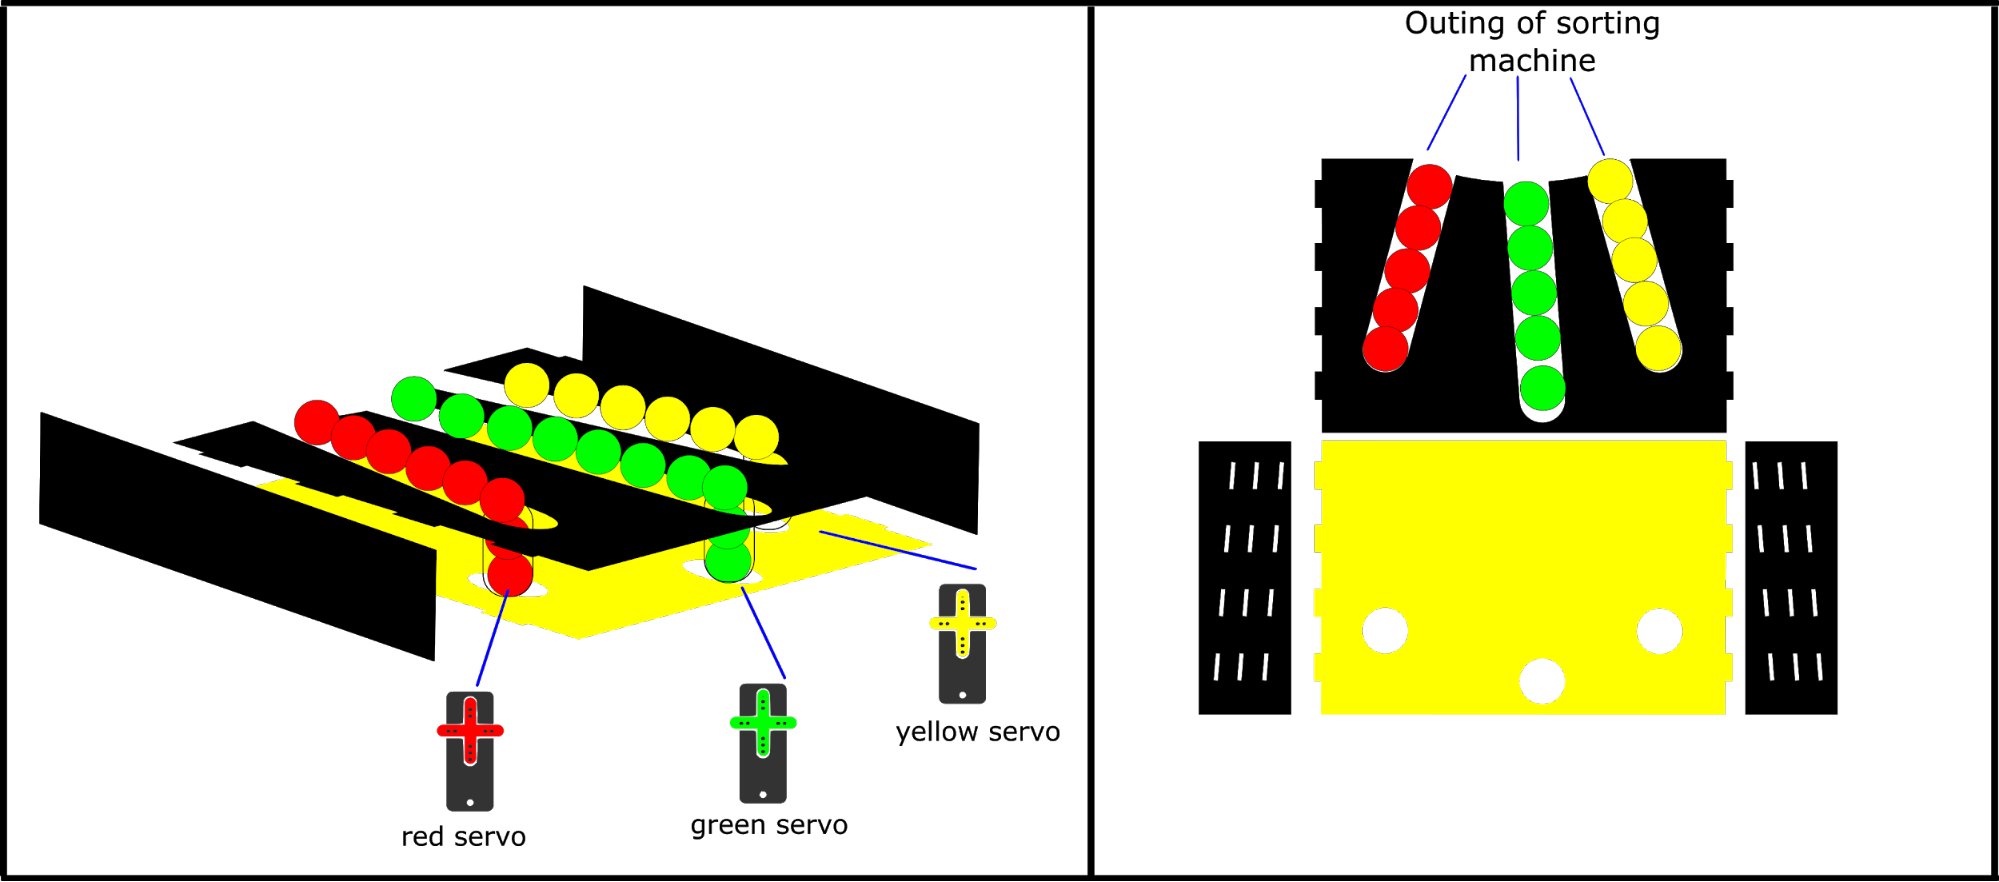
\includegraphics[width=100mm, height=35mm]{hard3}
    \centering
    \caption{Warehousing Part}
    \label{fig:hard3}
\end{figure}

\subsection{Collecting part}
This part is considered the third stage. The aim of this part is to take the product from the warehousing
stage and drop it down to the delivery box.\\
It has 3 servo motor as we have 3 colors in the warehousing, each servo motor moves with a specific
angle to drop down the ball into the box and return to the first angle to take the second ball ..etc\\
The base of this part is a (20 cm * 10 cm) and the height is 10 cm. Fig \ref{fig:hard4}

\begin{figure}[h]
    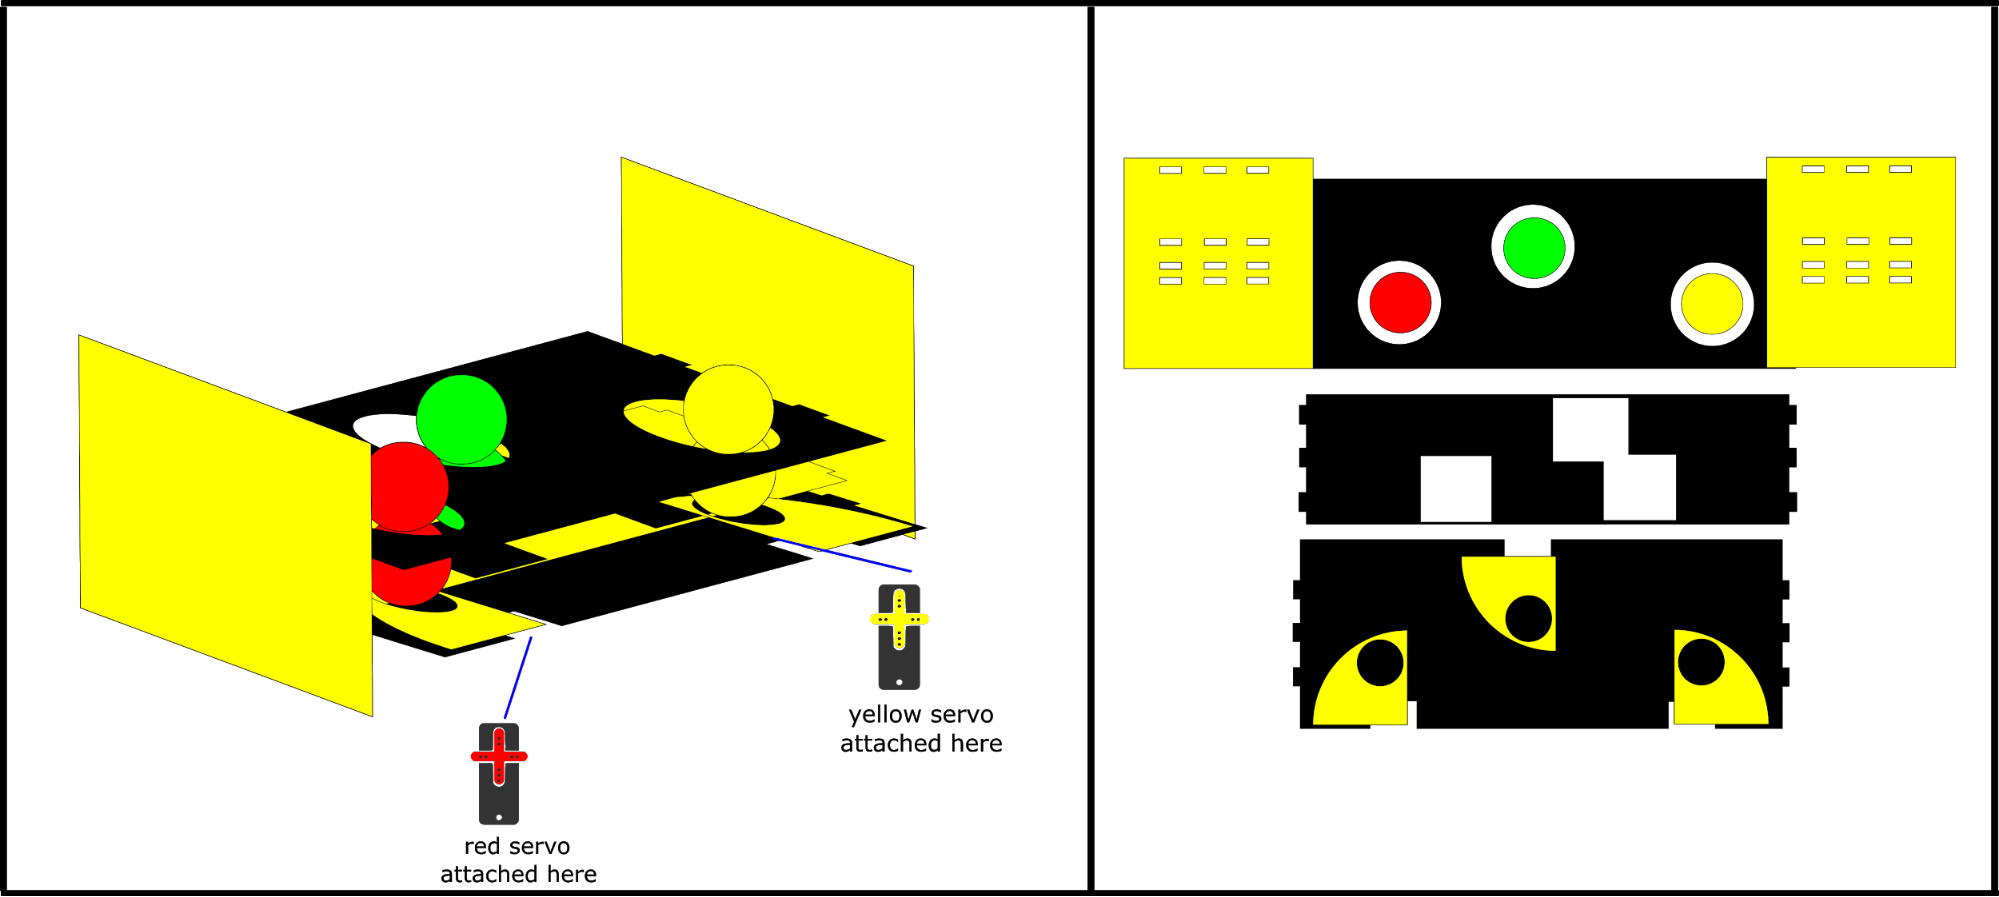
\includegraphics[width=100mm, height=35mm]{hard4}
    \centering
    \caption{Collecting Part}
    \label{fig:hard4}
\end{figure}

\subsection{The Base}
Finally, This part is made to collect the other parts on it.\\
The base of this part is a (40 cm * 35 cm) and the height is 10 cm. Fig \ref{fig:hard5}

\begin{figure}[h]
    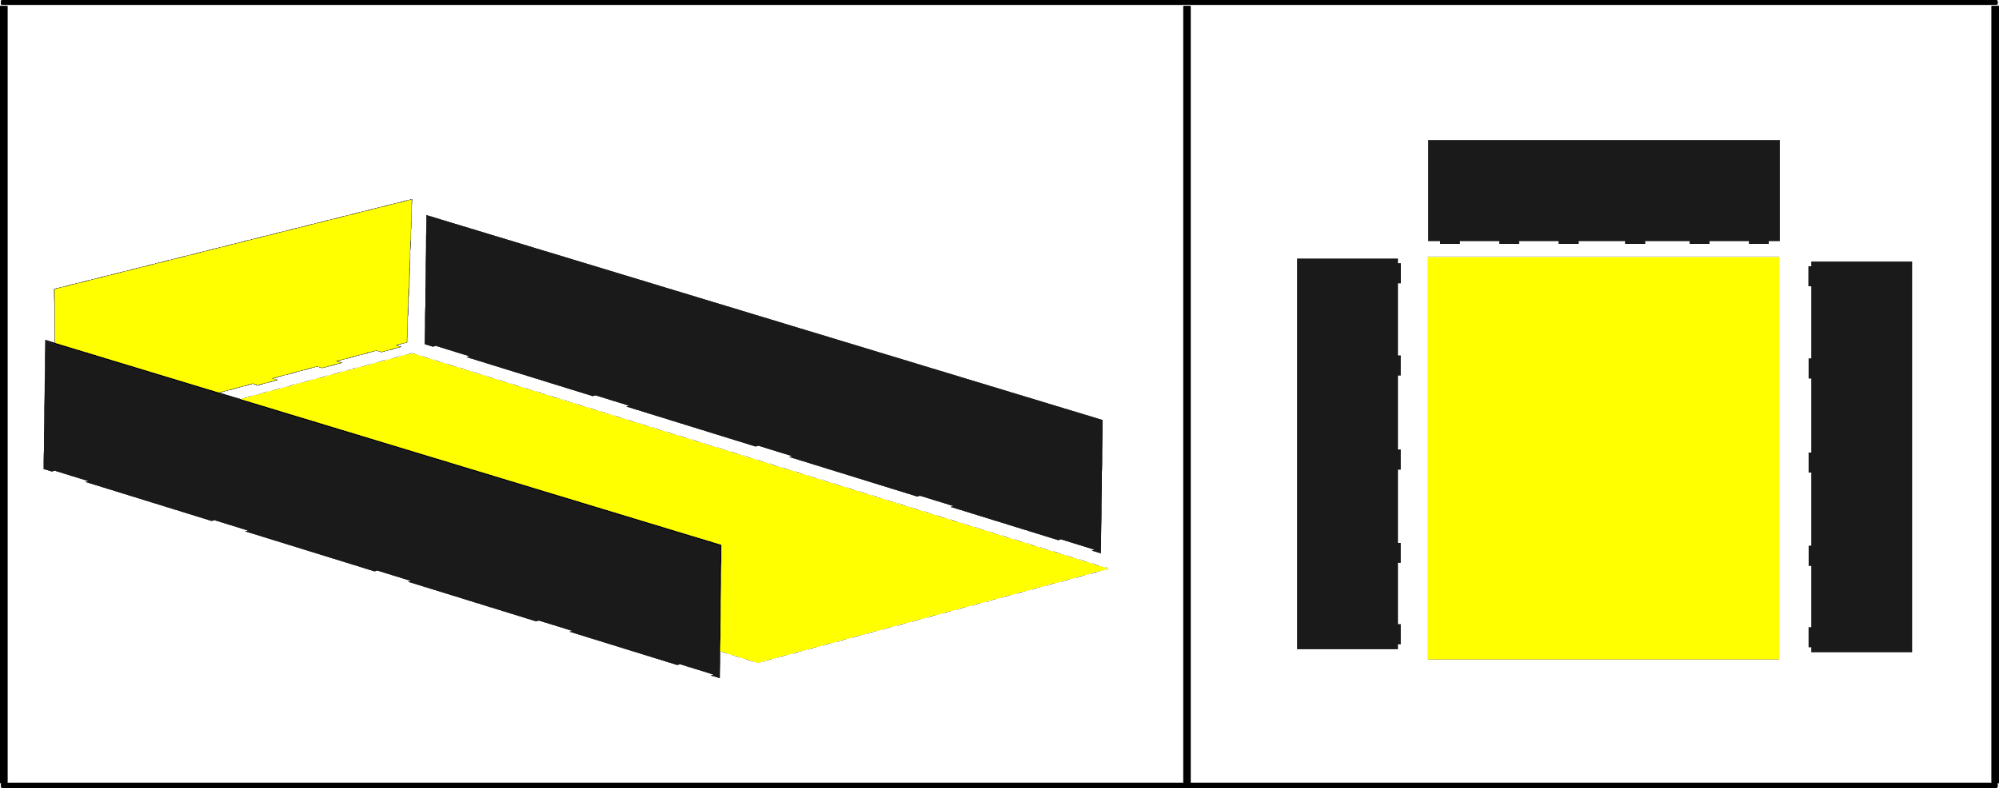
\includegraphics[width=100mm, height=35mm]{hard5}
    \centering
    \caption{The Base}
    \label{fig:hard5}
\end{figure}

\section{components used}

\begin{itemize}
    \item TCS230 RGB Color Sensor
    \item Servo Motor
    \item Arduino Uno
    \item Node MCU
\end{itemize}

\subsection{TCS230 RGB Color Sensor}

\begin{wrapfigure}{r}{0.25\textwidth}
    \begin{center}
      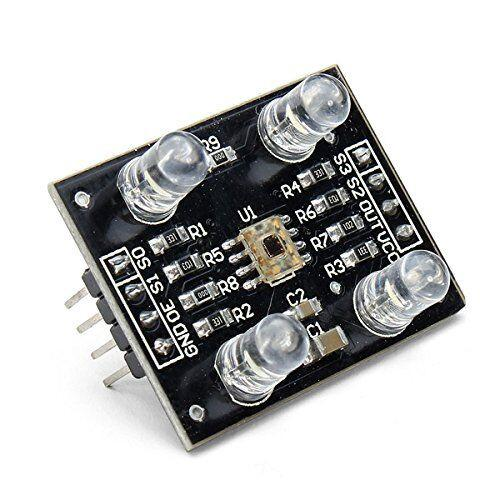
\includegraphics[width=0.25\textwidth]{node}
    \end{center}
  \end{wrapfigure}

The TCS230 senses color light with the help of an 8*8 array of
photodiodes.\\
Then using a Current-to-Frequency Converter the readings from the
photodiodes are converted into a square wave with a frequency directly
proportional to the light intensity.\\
Finally, using the Arduino Board we can read the square wave output and
get the results for the color.\\\\

\begin{center}
    
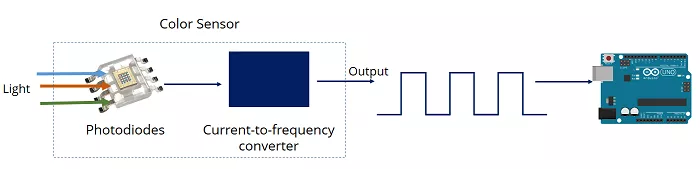
\includegraphics[width=\linewidth]{color_sensor}
\end{center}

\begin{wrapfigure}{r}{0.25\textwidth}
    \begin{center}
      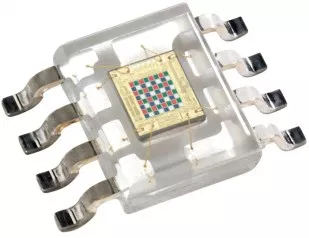
\includegraphics[width=0.25\textwidth]{node2}
    \end{center}
  \end{wrapfigure}

  If we take a closer look at the sensor we can see how it detects various colors.
  The photodiodes have three different color filters.\\
  Sixteen of them have red filters, another 16 have green filters, another 16 have
  blue filters and the other 16 photodiodes are clear with no filters.\\\\\\

  The 16 photodiodes are connected in parallel. Using the two control pins S2 and S3 we can select
which of them will be read. For example, if we want to detect red color, we can just use the 16 red
filtered photodiodes by setting the two pins to LOW logic level according to the table.\\\\
The sensor has two more control pins, S0 and S1, which are used for scaling the output frequency.
The frequency can be scaled to three different preset values of 100\%, 20\%, or 2\%.
This frequency-scaling function allows the output of the sensor to be optimized for various frequency
counters or microcontrollers.

\begin{center}
    
    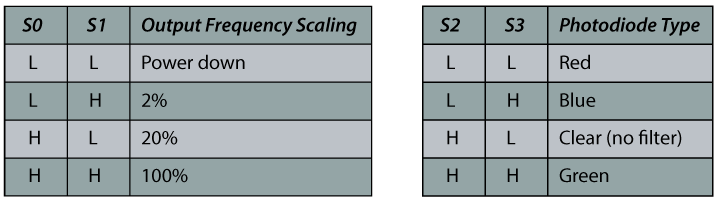
\includegraphics[width=\linewidth]{node_data}
    \end{center}

\subsection{Servo motor}

\begin{wrapfigure}{r}{0.25\textwidth}
    \begin{center}
      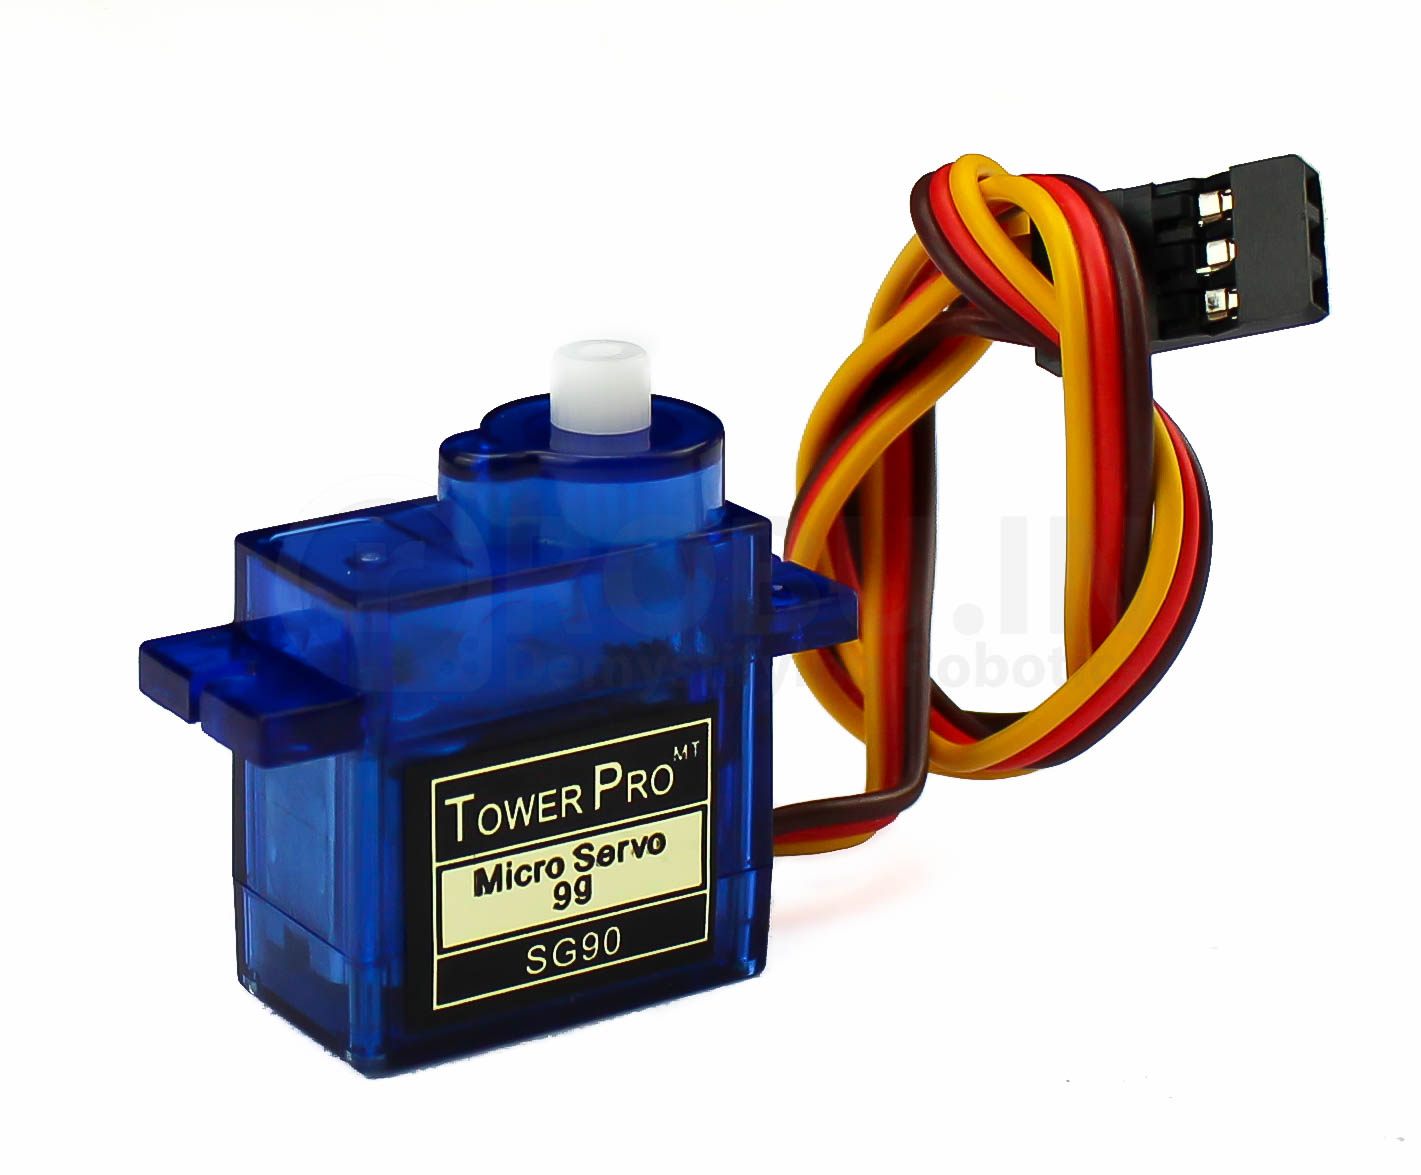
\includegraphics[width=0.25\textwidth]{servo}
    \end{center}
  \end{wrapfigure}

A servo motor is a closed loop servomechanism that uses position feedback to
control its motion and final position. The input to its control is a signal
(analog or digital) representing the position commanded for the output shaft.\\\\
Controlling a servo motor directly from the Arduino is quite easy. However,
a servo motor may require significantly more current than the Arduino can
provide. So we used an external power supply to provide the required current
to the servo motor.\\\\
We used 2 servo motors in the sorting part (upper and lower servo) and 3
servo motors in the collecting part (red, green, and yellow servo).

\subsection{Arduino Uno}

\begin{wrapfigure}{r}{0.25\textwidth}
    \begin{center}
      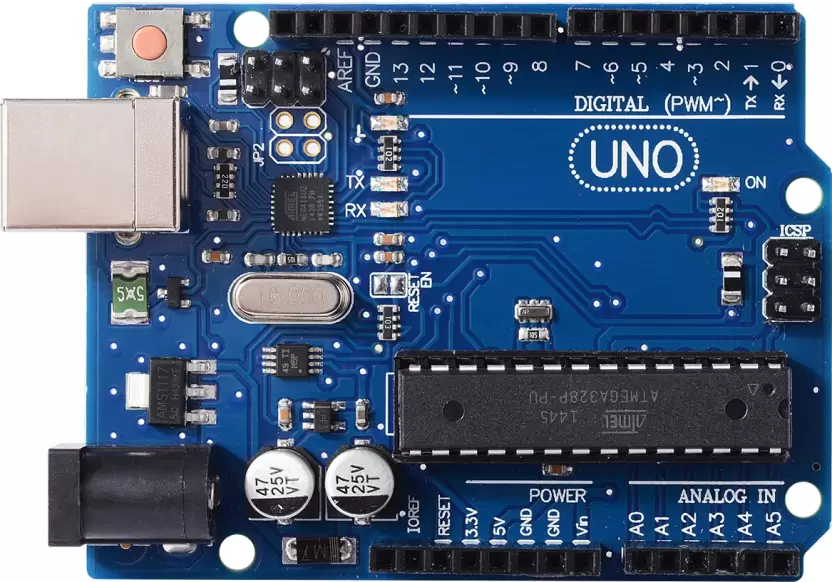
\includegraphics[width=0.25\textwidth]{arduino1}
    \end{center}
  \end{wrapfigure}

  Arduino Uno is a microcontroller board based on the
  ATmega328P. It has 14 digital input/output pins (of which 6
  can be used as PWM outputs), 6 analog inputs, a 16 MHz
  quartz crystal, a USB connection, a power jack, an ICSP
  header, and a reset button.\\\\
  It contains everything needed to support the microcontroller;
  simply connect it to a computer with a USB cable or power it
  with an AC-to-DC adapter or battery to get started.\\\\
  We used Arduino Uno to run the sensor and to control the 2
  servo motors of the sorting part\\


  \begin{figure}[h]
    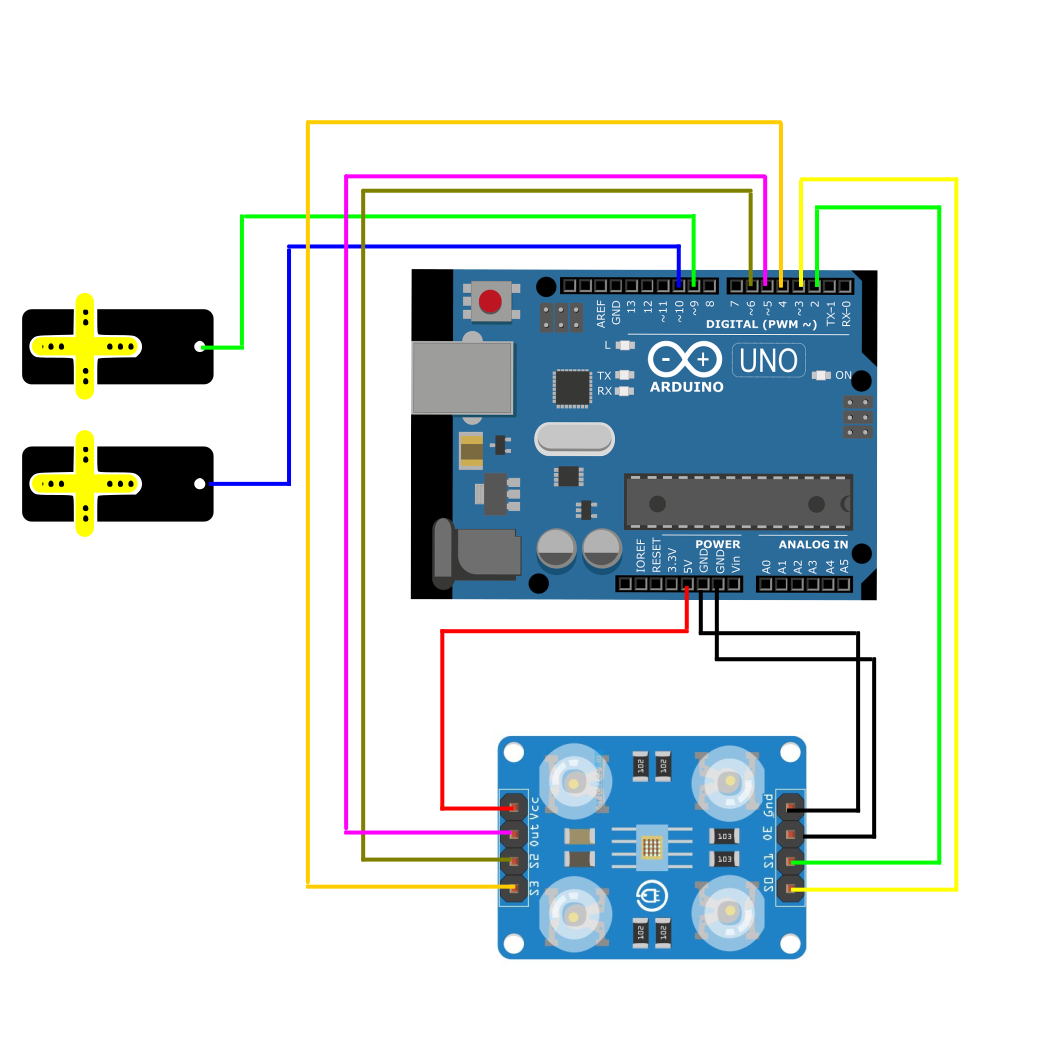
\includegraphics[width=\linewidth]{arduino2}
    \centering
    \caption{Sorting Connection diagram}
    \label{fig:arduino2}
\end{figure}

\subsection{Node MCU}

\begin{wrapfigure}{r}{0.25\textwidth}
    \begin{center}
      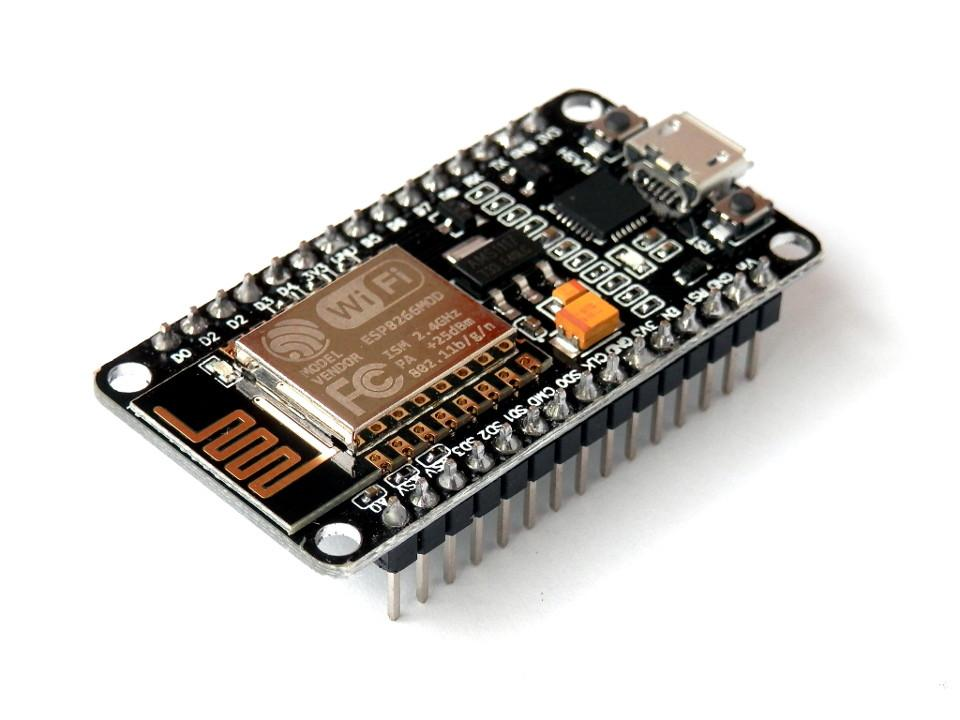
\includegraphics[width=0.25\textwidth]{mcu1}
    \end{center}
  \end{wrapfigure}

  In our project, we need wireless communication to connect the Arduino
to the web application, so we used NodeMcu.\\\\
It is an open source IoT platform. It includes firmware which runs on
the ESP 8266 Wi-FI SOC.\\\\
We also used it to control the 3 servo motors of the collecting part as it
has PWM output pins.\\\\
We used serial communication to connect the Arduino to the NodeMcu
to exchange the data between them.\\

\begin{figure}[h]
    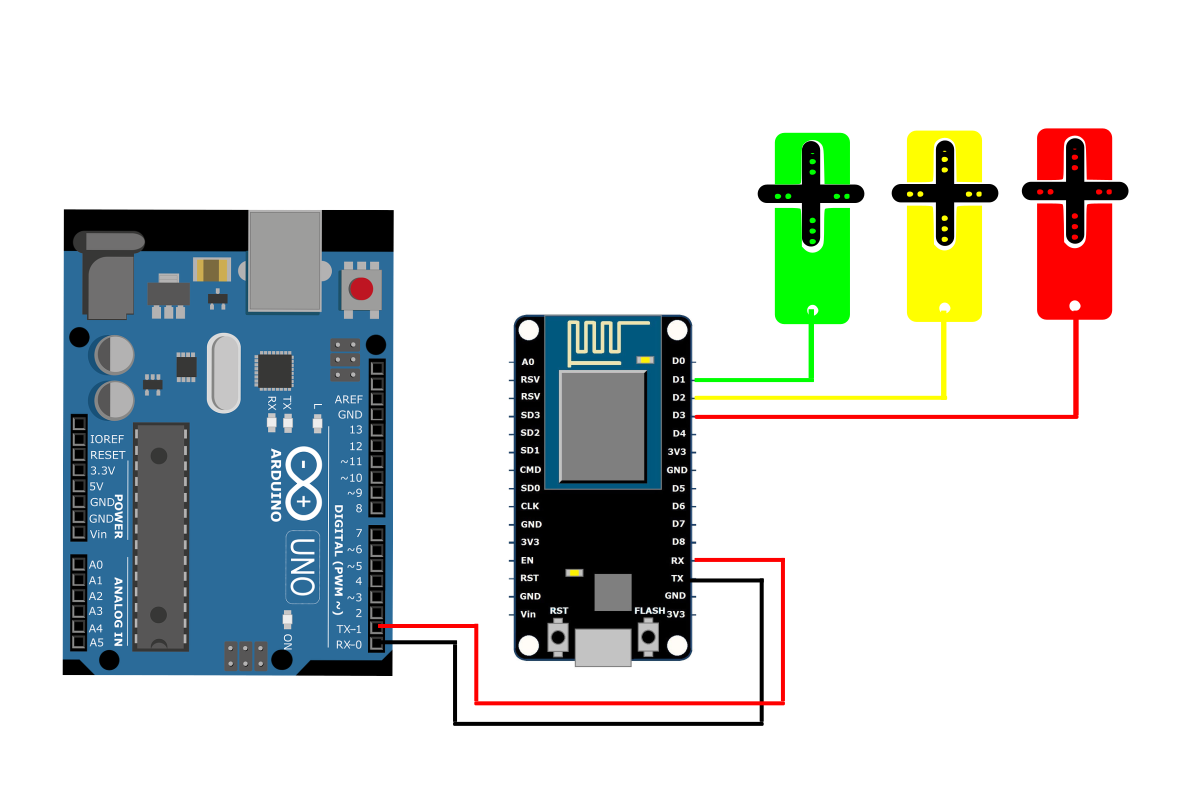
\includegraphics[width=\linewidth]{mcu2}
    \centering
    \caption{Collecting Connection diagram}
    \label{fig:arduino2}
\end{figure}


\chapter{Software}

The software will provide a way to have control over the project and visual feedback of the system
overall and offers the products for sale through an online market.\\\\
The software system is divided into three parts
\begin{itemize}
    \item Server Side
    \item Client Side
    \item Mobile Aoolications
\end{itemize}

\section{Server Side}

\begin{center}
    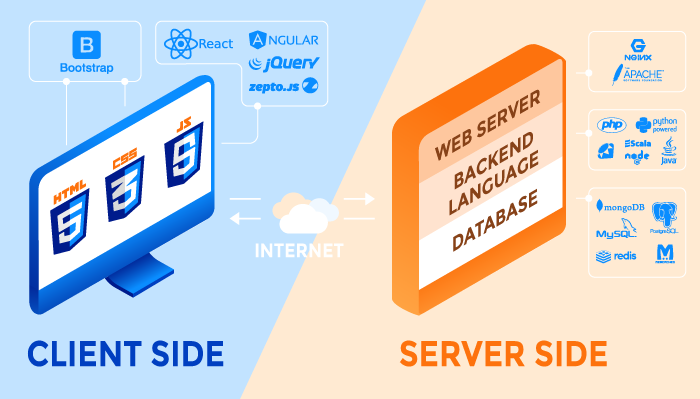
\includegraphics[width=\linewidth]{server}
  \end{center}

  A server is a computer program or a device that provides functionality for other programs or devices,
called "clients". This architecture is called the client-server model. A server should be reachable from
a user's local computer, smartphone, or other devices. Operations may be performed in server-side
because they require access to information or functionality that is not available on the client, or
because performing such operations on the client side would be slow, unreliable, or insecure.\\\\
The Factory software is built upon this architecture, where the server provides an API to be accessed
by the clients using it.\\\\
The server also talks to the hardware using Socket for real-time, bi-directional communication
between clients (Node MCU in our case) and the server.\\\\
The server API provides
\begin{itemize}
    \item User Authentication, it will validate the user signing in the system
    \item User Data, it will get the data related to the user
    \item Getting the orders
    \item Sending the order to the hardware
\end{itemize}

All connections to the database are done using the server. The database used is firebase, which is a
cloud database solution that helps to quickly develop high-quality apps and grow the business. Data is
stored as JSON and synchronized in real-time to every connected client.\\\\
The server uses the database to store data about
\begin{itemize}
    \item Users of the system
    \item Clients
    \item Orders
    \item Drivers (Which we will discuss their purpose later in the book)
\end{itemize}

\section{Client Side}

\begin{center}
    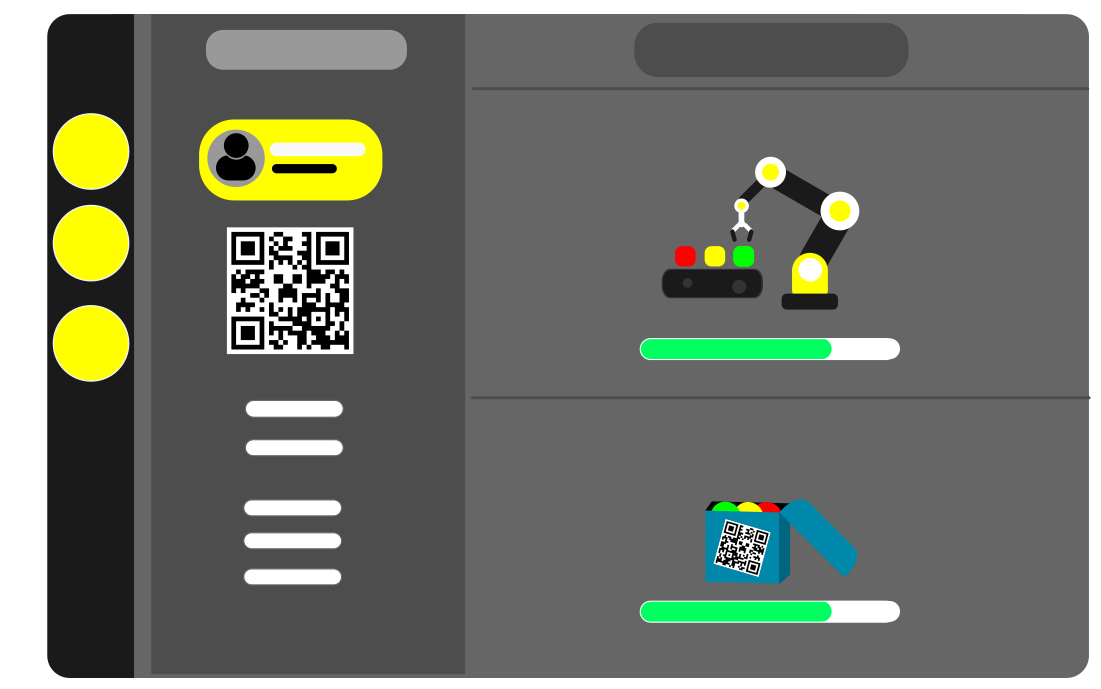
\includegraphics[width=\linewidth]{client}
\end{center}
The client-side refers to a computer application, such as a web browser, that runs on a user's local
computer, smartphone, or other devices, and connects to a server as necessary.\\\\
Client side will provide a way for users of the business to log into the system, control the hardware
and have an overview of the overall business, like the orders made by customers and the state of the
orders.\\\\
The client app will offer these operations
\begin{itemize}
    \item Display the orders in details
    \item Talk to the server API
    \item Sending orders to the hardware via server API. Sending order to hardware to start the
    manufacturing and prepare process, as orders aren’t permitted to start without a user manually
    evaluating the order and then send the order to the hardware
    \item Monitor the order process. Monitor the order allows the process to have feedback on how the
    process is doing or if there is any problem with the system
\end{itemize}

The client app is built using Vue.js which is a progressive framework for building user interfaces and
single web applications.\\\\
Vue.js has these features that will make the developing simpler
\begin{itemize}
    \item Utilizes a virtual DOM
    \item Provides reactive and composable view components
    \item Maintains focus in the core library, with concerns such as routing and global state
    management handled by companion libraries
\end{itemize}


\section{Client App}

Smartphones are no longer just devices for calls, they are also used to send multimedia messages such
as pictures, videos, and emails. Due to the enormous potential of smartphones, these capabilities can
be exploited by multiple applications that benefit the user, so we tried to make simple and useful
applications to our hardware project.\\\\
The aim of this client android application is providing an easy way to make an order from the factory
and track the order until it reaches the customer's location. It also displays all the orders from the
client.\\\\

\textbf{Tools used}
\begin{itemize}
    \item Software Requirements: Android studio, Java
    \item Database: Firebase
\end{itemize}
\textbf{Features}
\begin{itemize}
    \item Provides users authentication
    \item Makes orders
    \item Tracks order location by using google map
    \item Receives notifications about the order
    \item Checks the Qr code of the order
    \item Displays all orders
    \item Provides statistics profile
\end{itemize}

\begin{figure}[h]
    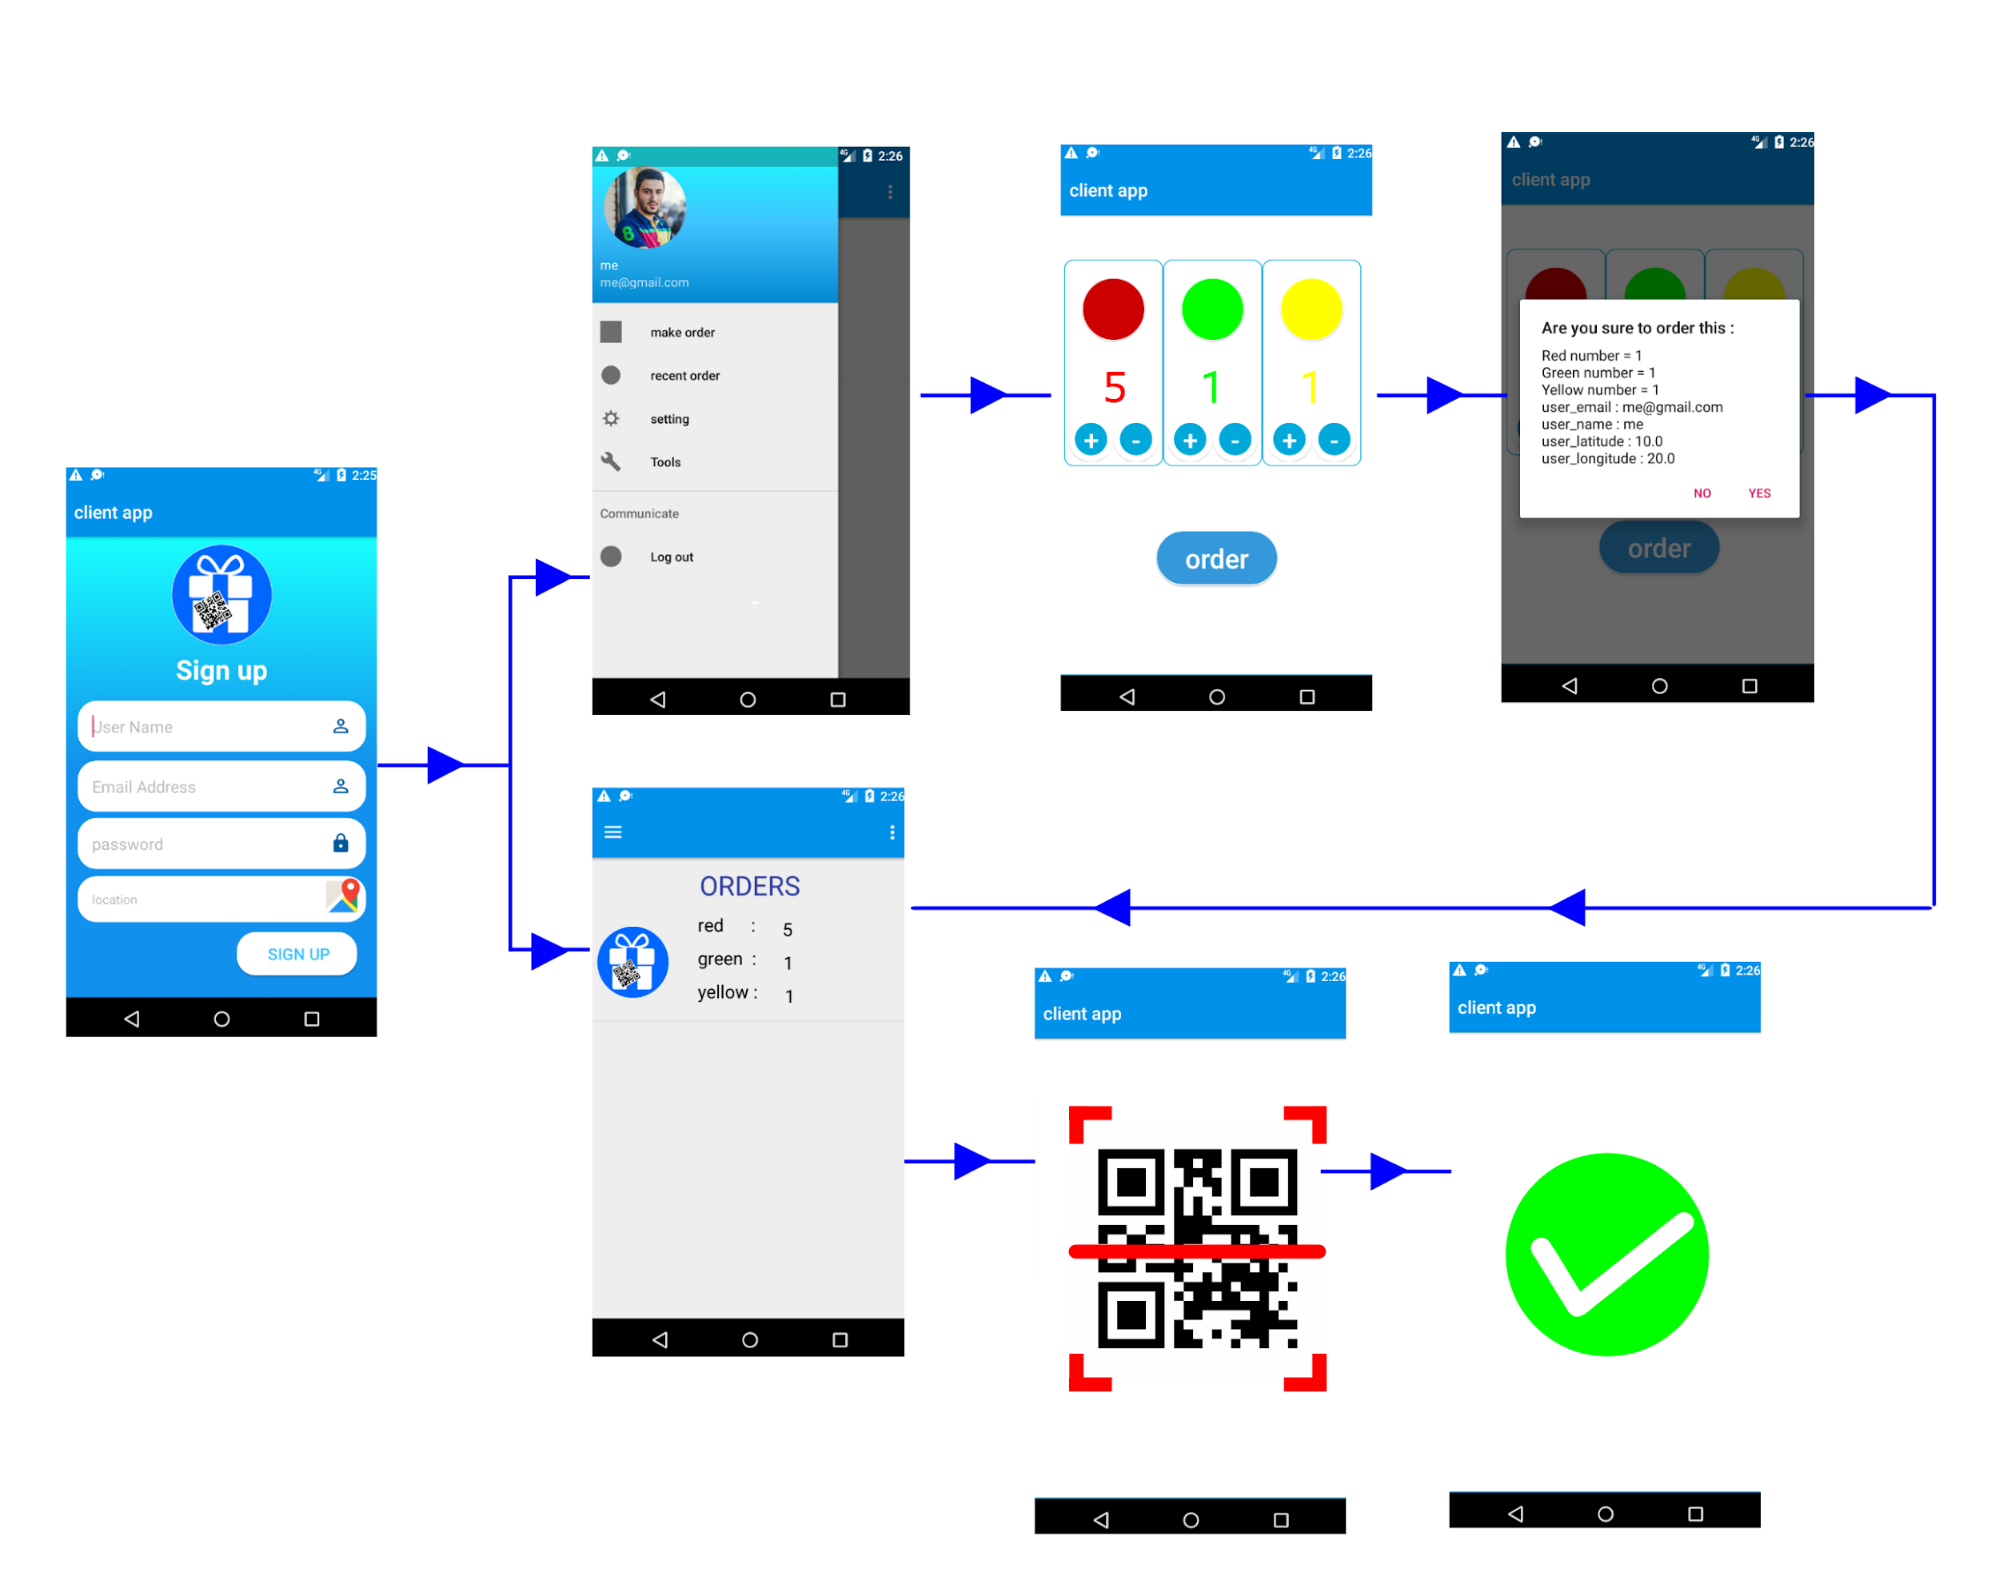
\includegraphics[width=\linewidth]{blue1}
    \centering
    \caption{Process Flow of the Client Application}
    \label{fig:blue1}
\end{figure}

\subsection{QR Code}
A QR code (quick response code) is a type of 2D barcode that is used to provide easy access to
information through smartphones.\\\\
In our android applications, we need to store the order of each customer and the location of the
customer.\\\\
We stored the data we need in a JSON object to extract the data from it in an easy way.\\\\

\par\vspace {4cm}
\begin{wrapfigure}{r}{0.5\textwidth}
    \begin{center}
      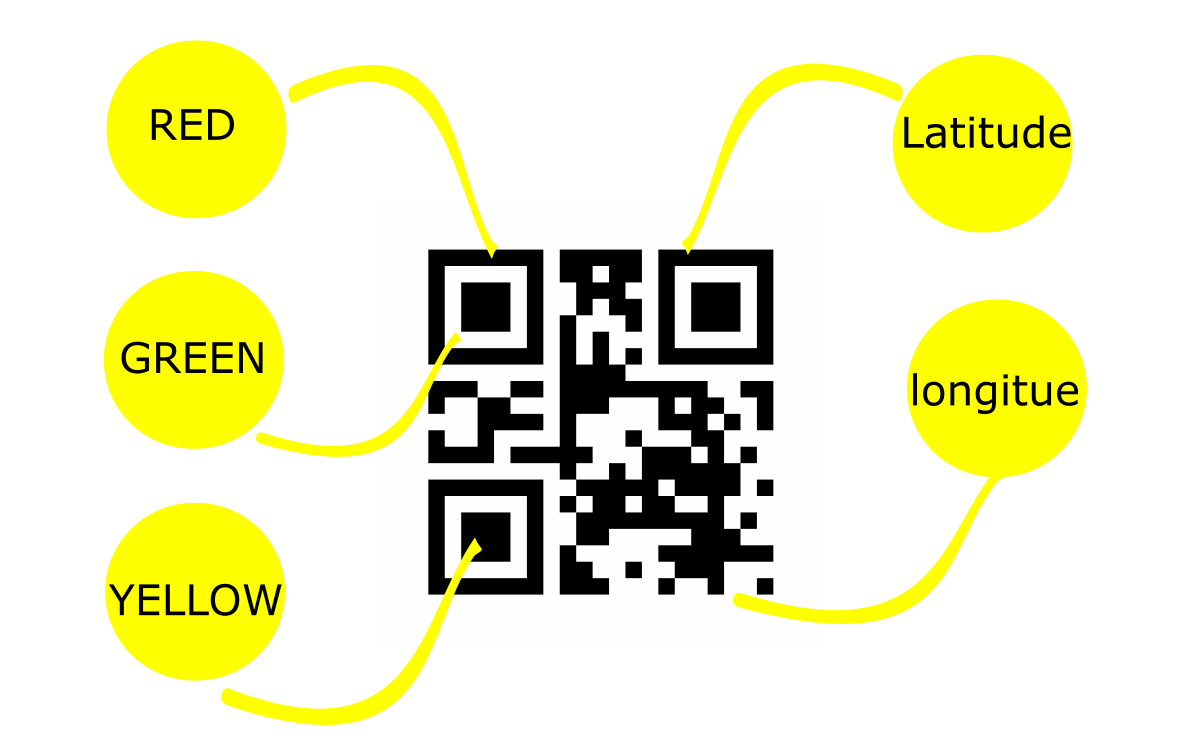
\includegraphics[width=0.5\textwidth]{qr}
    \end{center}
  \end{wrapfigure}

\textbf{For example}\\
\small \{
    \begin{adjustwidth}{2cm}{}
    \small Red : 5,\\
    \small Green : 1,\\
    \small Yellow : 1,\\
    \small Latitude : 30.35,\\
    \small Longitude: 30.59\\
    \end{adjustwidth}

    \small \}\\\\\\

    As the order consists of three products (red, green, and
    yellow) and the location of the customer (latitude and
    longitude) that our application uses to get the location on
    google maps.

\subsection{Process Flow}

The process flow of the client application during making the order Fig \ref{fig:blue2}
\begin{itemize}
    \item The client makes an order
    \item The firebase sends the notification order to the web app to collect it
    \item The web app collects the order and puts it in a box with a printed QR code
    \item The delivery service takes the order and delivers it to the client
    \item The client scans the QR code of the order
    \item The client app displays the contents of the box
\end{itemize}

\begin{figure}[h]
    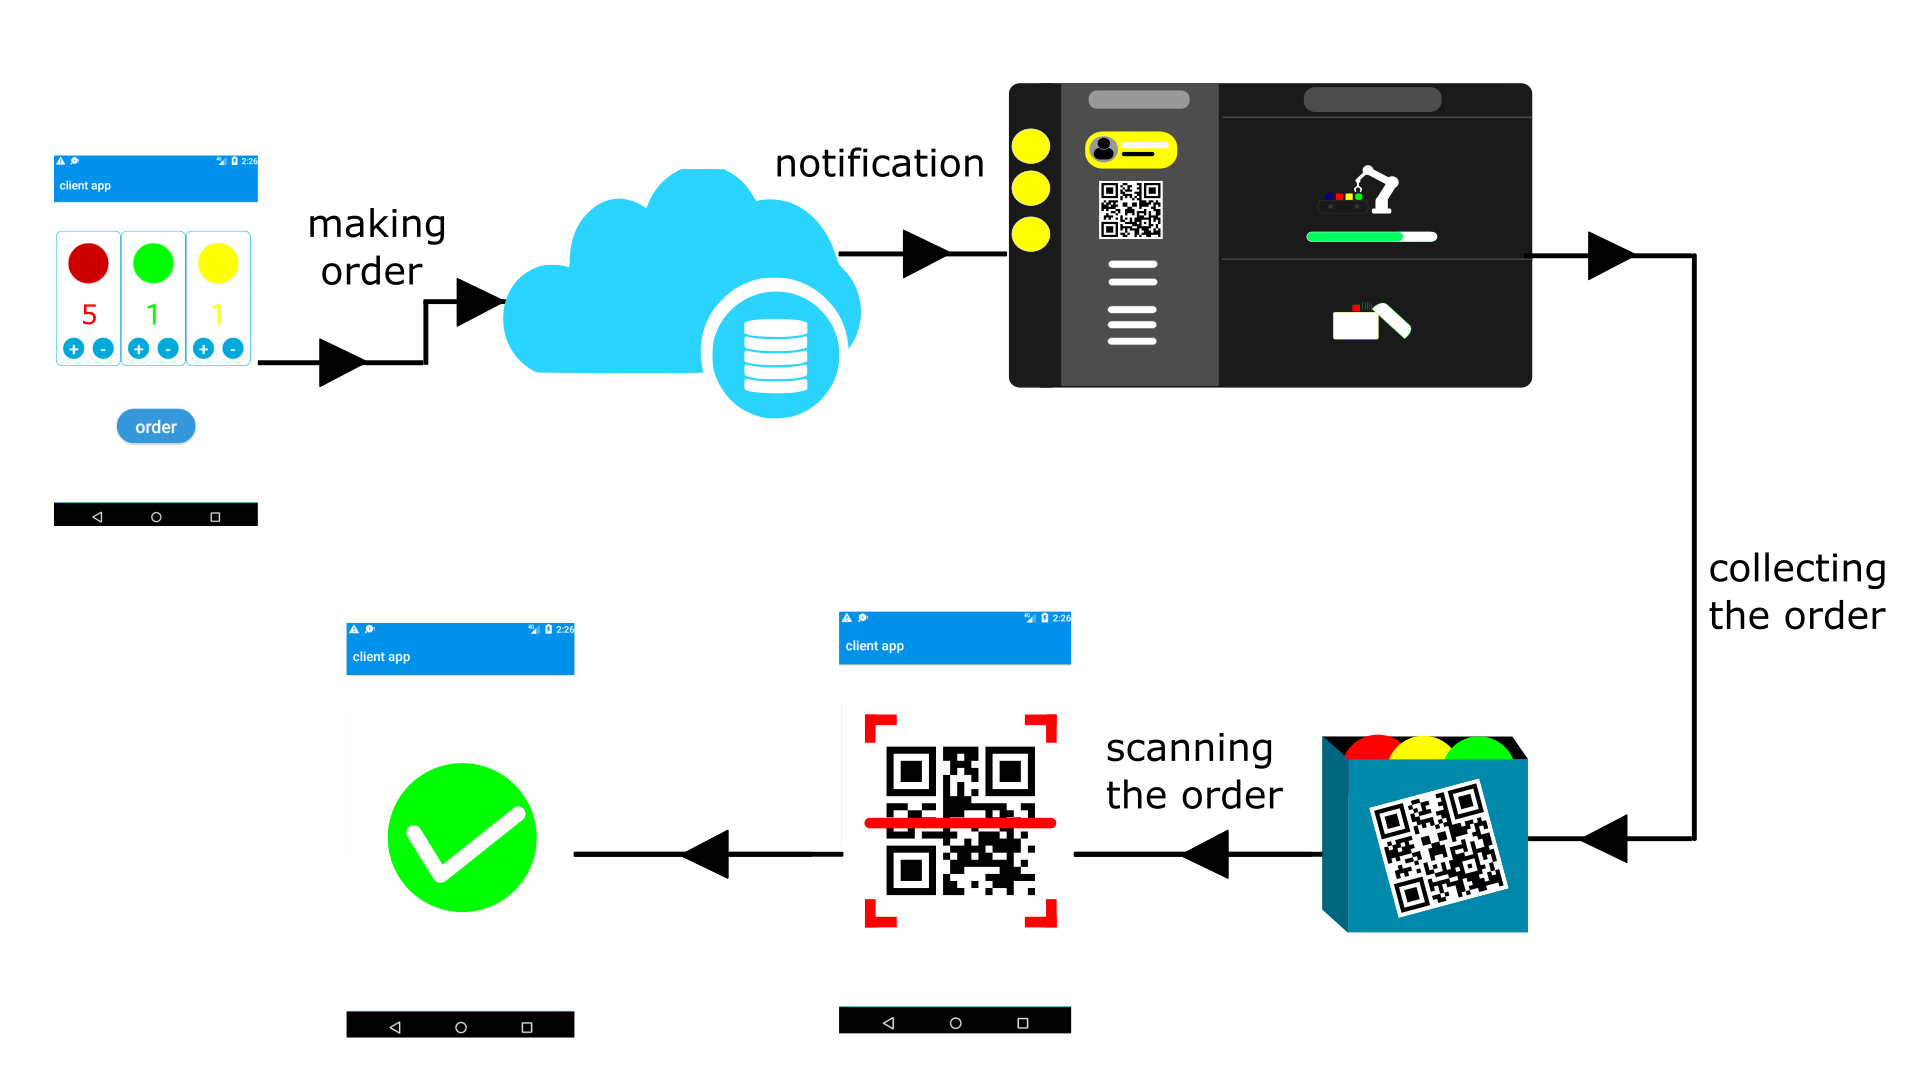
\includegraphics[width=\linewidth]{blue2}
    \centering
    \caption{Making Order Flow}
    \label{fig:blue2}
\end{figure}



\section{Important screens}
\begin{itemize}
    \item Getting the location of the client by using google maps
    In the registration form, when the client presses on the icon of google maps, the app will open
    google maps screen and store the location of the client
    \item Scanning the Qr code of the order when receiving it, then the application will display the
    status of the order if it is the right or wrong order
\end{itemize}

\section{Driver App}

The aim of this driver android application is providing an easy way to get to the final destination of
the order on google maps then deliver it to the client\\\\

\textbf{Tools used}
\begin{itemize}
    \item Software Requirements: Android studio, Java
    \item Database: Firebase
\end{itemize}

\textbf{Features}
\begin{itemize}
    \item Real-time communication
    \item Users authentication
    \item Checks the QR code of the order
    \item Displays the location of the customer
    \item Displays all targeted locations
\end{itemize}


\begin{figure}[h]
    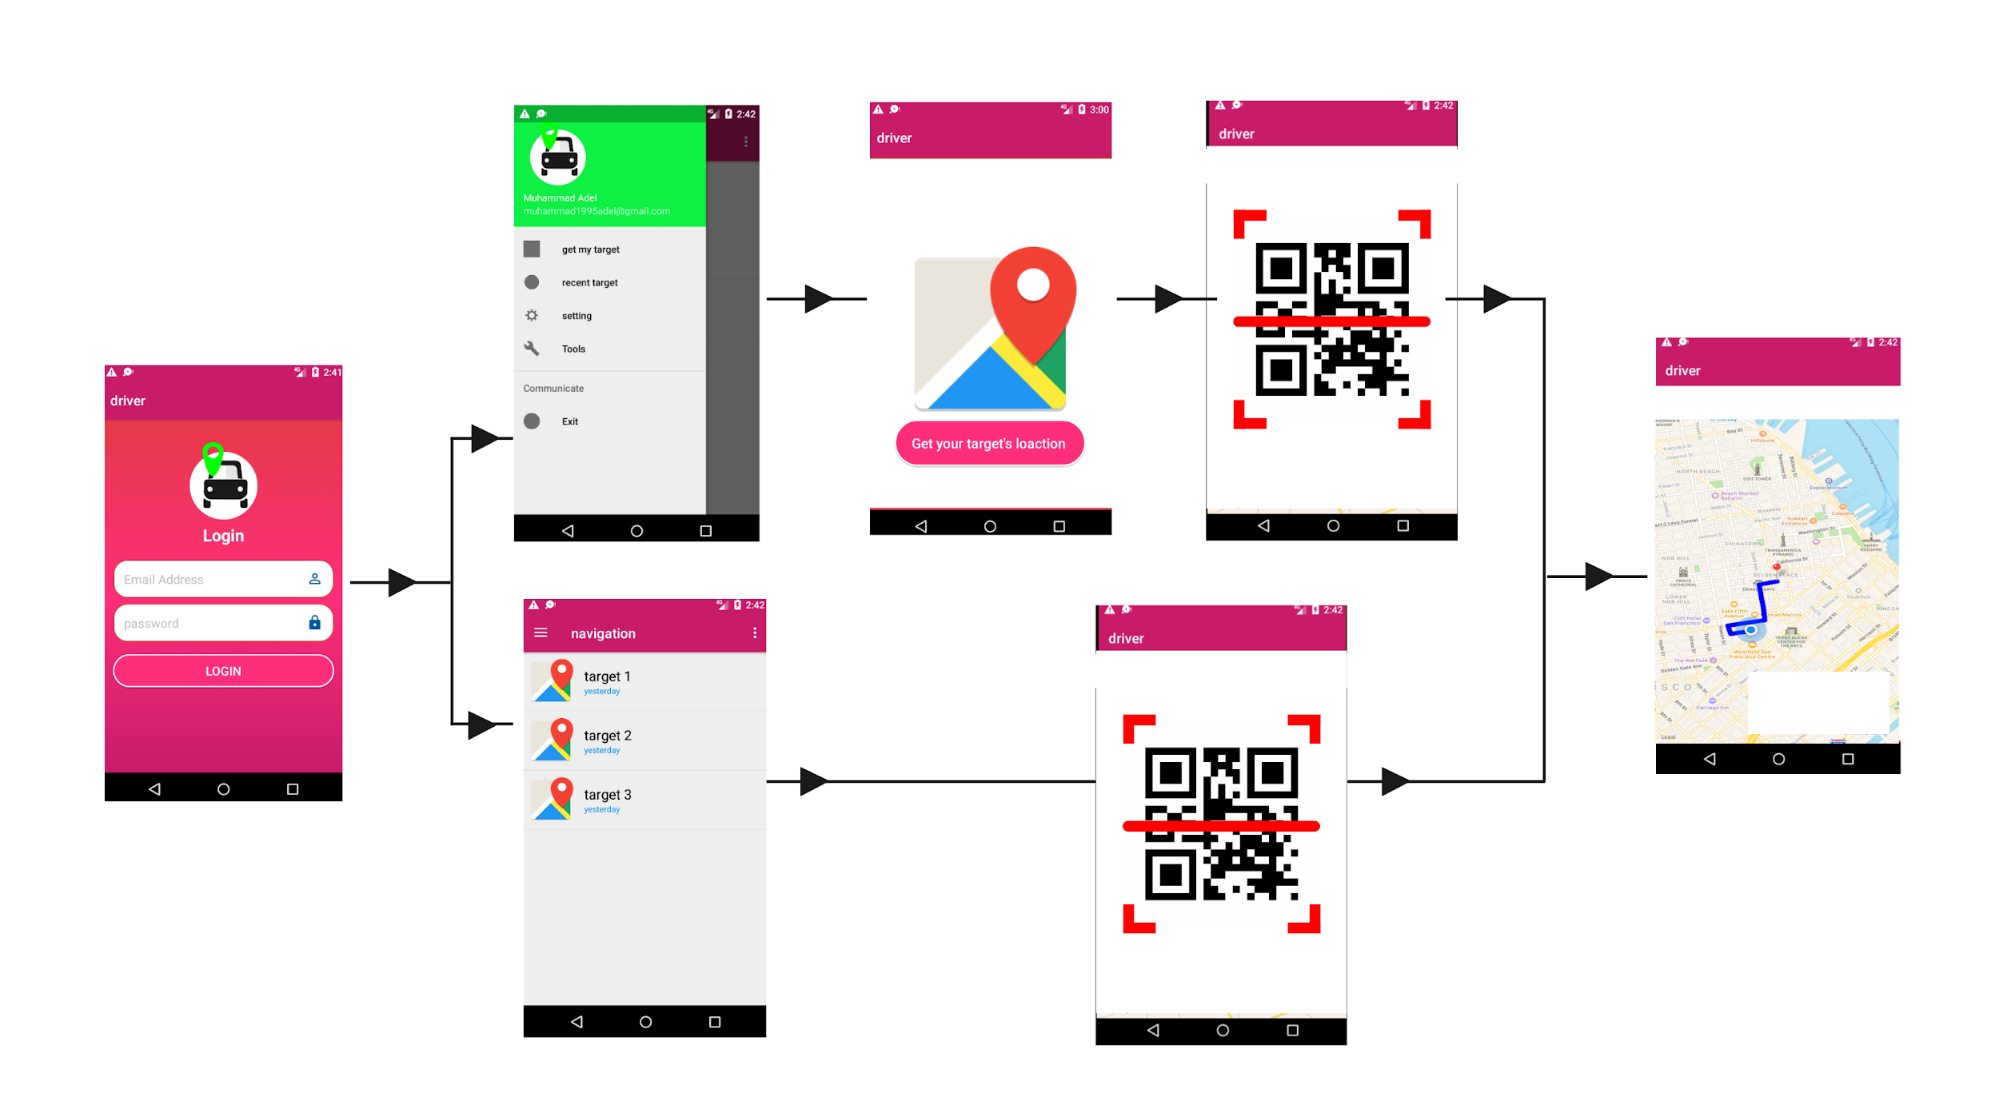
\includegraphics[width=\linewidth]{red1}
    \centering
    \caption{Process Flow of the Driver Application}
    \label{fig:red1}
\end{figure}

\subsection{Process Flow}

The process flow of the driver application during making the order Fig \ref{fig:blue2}
\begin{itemize}
    \item The web app sends a notification to the driver app after finishing the order
    \item The driver scans the QR code of the order
    \item The driver app displays the destination of the order on google maps and draws the shortest
    route between the two locations
    
\end{itemize}

\begin{figure}[h]
    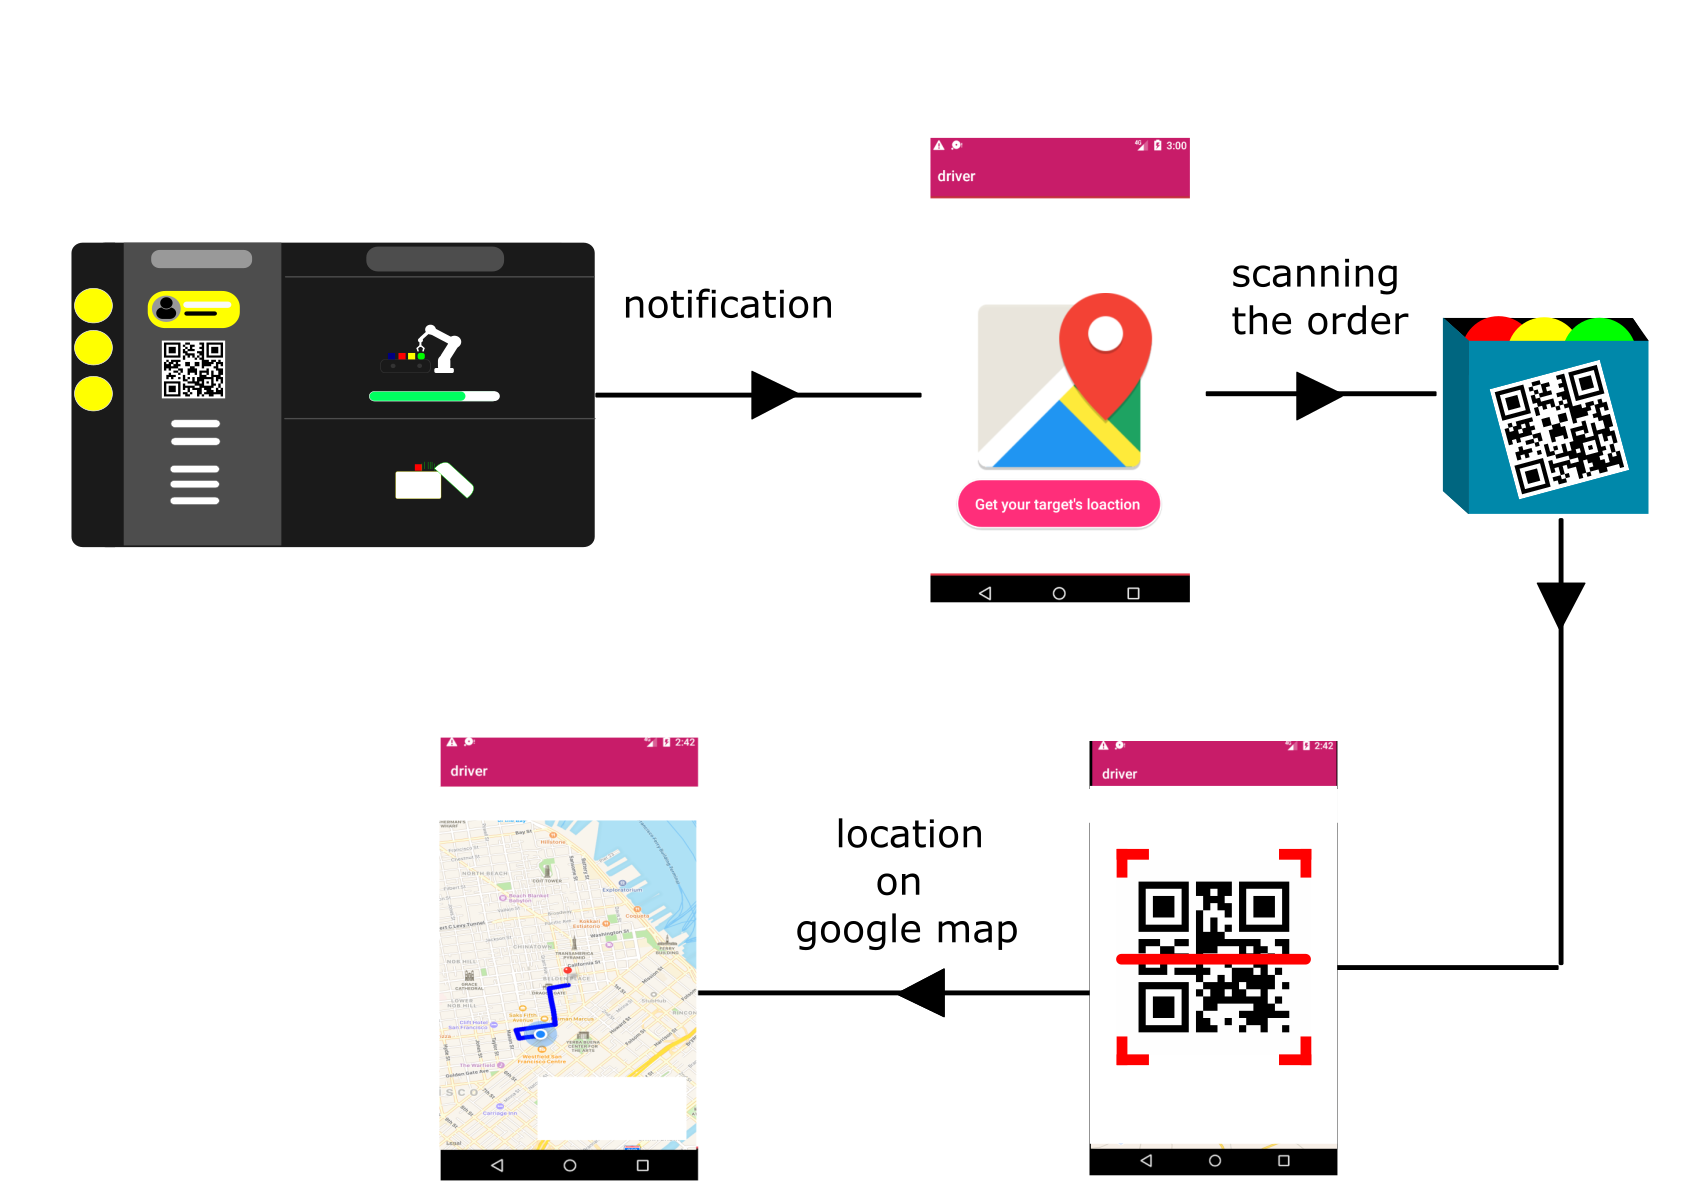
\includegraphics[width=\linewidth]{red2}
    \centering
    \caption{Finishing Order Flow}
    \label{fig:red2}
\end{figure}



\subsection{Important screens}
\begin{itemize}
    \item Scanning the QR code of the order, then the application will get the latitude and longitude of
    the customer and pass it to google maps activity to display the shortest path between the
    driver and the customer.
\end{itemize}